\documentclass[]{article}
\usepackage{graphicx}
\usepackage{url}
\usepackage{fullpage}
%opening
\title{\textbf{DRAM Capacity Growth}}
\author{Adam Sumner \\ ECE 485}
\date{}

\begin{document}

\maketitle

\section{Updated Graph}

\begin{figure}[h!]
\centering
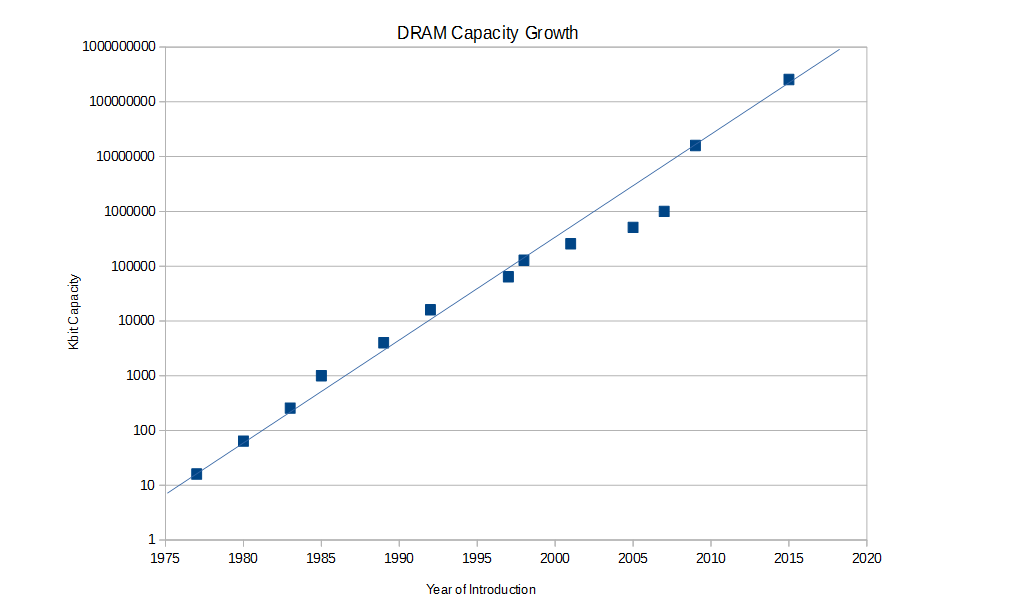
\includegraphics[width=1\linewidth]{graph}
\caption{Updated DRAM Capacity Trend Graph}
\label{fig:graph}
\end{figure}

Sources: 
\begin{itemize}
	\item \url{http://en.wikipedia.org/wiki/Dynamic_random-access_memory}
	\item \url{http://www.pwc.com/gx/en/technology/mobile-innovation/dram-memory-device-innovation.jhtml}
	\item \url{http://www.singularity.com/charts/page58.html}
\end{itemize}
~\\
~\\
It is clear from the graph that DRAM capacity follows Moore's law. Through my research I found that the bit/dollar price increased logarithmically, which coincides with the data I found that the capacity is increasing at a logarithmic rate. 

\end{document}
